\section{Introduction}


A key tenet in economics is that the degree to which firms should be
willing to invest in a given project depends crucially on the required
rate of return to capital: A price-taking firm should install just
enough capital so that its marginal product of capital, $MPK_i$,
equals the required rate of return to capital, $r_i$,
\begin{equation}
  MPK_i=\underbrace{r^f+RP_i}_{r_i}.
  \label{eq_one}
\end{equation} 
This equation is the point of departure for many classic questions in
economics. Students of asset pricing are taught that a firm's $r_i$
has two components; a risk-free part, $r^f$, and a risk-premium,
$RP_i$, that depends on the firm's risk characteristics. One of the
classic puzzles in asset pricing asks why $RP_i$ is so large relative to
$r^f$ (the equity premium puzzle). Monetary economists are interested
in the Federal Reserve's power to increase or decrease investment by
manipulating $r^f$, while students of economic growth often take
differences in $MPK_i$ as a measure of inefficiencies in the
allocation of capital across countries, sectors, and firms.

In this article we argue that recent insights from the study of
currency risk premia have important lessons for how we should think
about Equation \eqref{eq_one}, and by extension, for its key
applications in asset pricing, macroeconomics, and economic growth.
The simplest, and perhaps and most important, of these lessons is that
countries differ dramatically in their risk-free interest rates. These
differences in risk-free interest rates are large (on the same order
of magnitude as the equity premium puzzle), appear to be highly
persistent over time (lasting for decades rather than years), and
cannot be explained by predictable depreciations, government default,
or differences in inflation rates. Instead, these differences in
interest rates appear intimately linked to the risk characteristics of
the country's exchange rate, and to its exchange rate regime.

\begin{figure}
  \centering
  \caption{Risk-free Interest Rates}
  \includegraphics[width=0.7\textwidth]{Exhibits/Figure_FP12M_JPYNZD.pdf}
  \label{fig:fp}
\end{figure}
Figure \ref{fig:fp} shows the difference in the risk-free interest
rates of the New Zealand Dollar and the Japanese Yen as an example (we
will discuss below how one can measure such risk-free rates and
compare them across countries). The figure shows that the New Zealand
dollar had a higher risk-free rate than the Japanese Yen in
\textit{every} month between January 1997 and December 2018. On average,
this difference was about 4.90pp on an annualized basis. When we
adjust for movements in exchange rates over the period, the difference
in returns on the two countries currencies is 4.39pp -- meaning that a
US investors who borrowed in Yen and lent in New Zealand Dollars on
average made a return of XX percent over this period. (For comparison,
the equity premium on US stocks was about XXpp during the same
period.)

We now know that such highly persistent differences in interest rates,
similar to those between New Zealand and Japan, are common in the
data, even among developed economies. These large differences in
interest rates do not appear to be equalizing over time and translate
into large differences in returns investors can earn when investing in
these currencies.

Why would $r^f$ differ permanently across countries? The emerging
consensus in the literature is that the most likely explanation are
currency risk premia -- the idea that some currencies are safer
investments than others.

A useful way of thinking about this problem is to take the perspective
of a retail investor in a third country, say in Hong Kong. As is
common in many countries, Hong Kong-based banks regularly offer
savings accounts denominated in multiple currencies, so that our
fictitious investor might have the option to invest in yen at a
deposit rate of 0.1\% or in New Zealand Dollars at a rate of 3.0\%.
How might she decide between these two options? Since both accounts
are with the same bank, any likelihood of sovereign default is
irrelevant. Similarly, our Hong-Kong based investor does not care
about inflation in these two faraway countries. Instead, the only
relevant factors for her choice between these two investment is the
difference in interest rates and the stochastic behavior of the yen-to
New Zealand dollar exchange rate.

Because changes in exchange rates are largely unpredictable over short
horizons, our investor should not expect either currency to depreciate
over the coming year, leaving only one relevant consideration:
covariance.\footnote{A regression of the Japanese Yen to New Zealand Dollar
exchange rate on their interest rate differential yields an R-squared of
0.XX} Which of the two currencies does our investor trust to
retain value in a possible recession or crisis? Intuitively, she might
think that Japanese yen are a safer bet -- and she would be right.

Along with a number of other so called ``safe-haven currencies,'' the
Japanese yen tends to appreciate relative to the New Zealand dollar
during large international recessions and crises. 
\begin{figure}[htp!]
  \centering
  \caption{New Zealand Dollar - Japanese Yen Exchange Rate}
  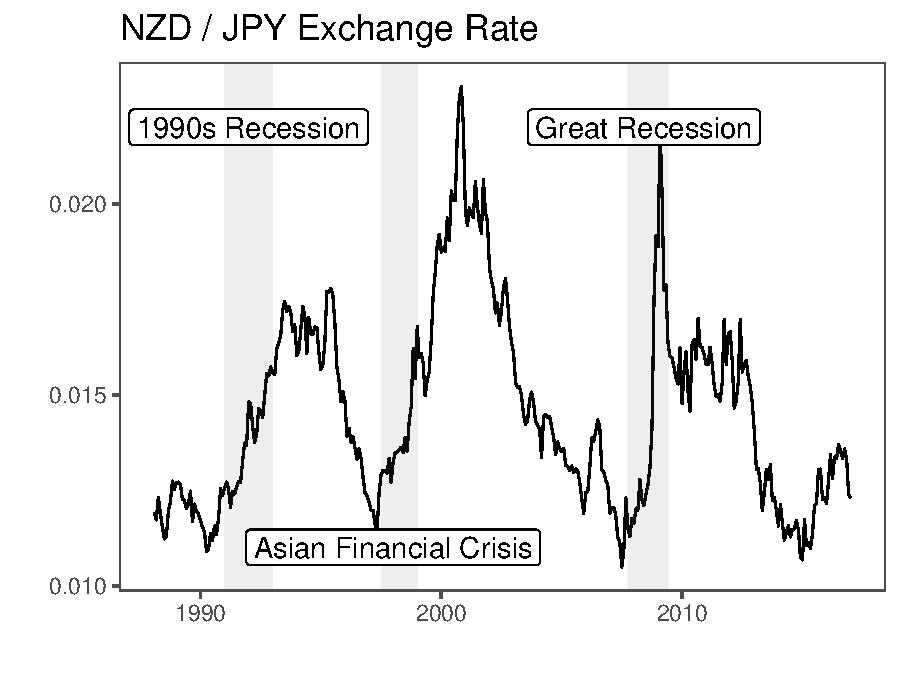
\includegraphics[width=0.7\textwidth]{Exhibits/Figure_FX_JPYNZD.pdf}
  \label{fig:spot}
\end{figure}
Figure
\ref{fig:spot} shows some evidendence of this pattern by plotting the New Zealand dollar - Japanese yen exchange
rate in terms of dollars per yen (so that an increase in the exchange rate
indicates yen appreciation). The shaded areas highlight three distinct
periods of global economic turmoil: The early 1990s recession (1990 -
1993), the Asian financial crisis (1997 - 1998), and the Great
Recession (2007 - 2009). In each of these periods, the yen appreciated
markedly against the New Zealand Dollar. If these appreciations during
periods of economic turmoil are part of a broader pattern, investors
should naturally consider the Japanese yen the safer currency -- and
if yen are a safer
store of value, it might make sense to accept a lower deposit rate.
That is, international investors might be willing to lend at lower
rates in currencies they expect to retain value when times are bad.


As it turns out, this simple intuition has a lot of support in the
data from international bond and derivatives markets. For example, a
seminal paper by \citet{LustigVerdelhan2007} shows that currencies
with low interest rates tend to appreciate when US consumption
growth is low, and depreciate when US consumption growth is high. That
is, there is direct evidence that currencies with low interest rates
appreciate when times are bad for US consumers, making these
currencies a safer store of value for investors.

In addition to this empirical evidence, the theoretical work on
currency risk has identified a number of theoretical reasons to expect
the emergence of safe-haven currencies and long-lasting differences in
interest rates. In a nutshell, persistent differences in countries' currency risk premia arise naturally in
a wide range of international macro models. For example,
\citet{Hassan2013} shows that simply allowing for some economies to be
larger than others within a standard international real business cycle
model is sufficient to generate long-term differences in interest
rates between countries, because the currencies of larger countries
tend to appreciate when world-wide output is low. That is, even within
the most canonical, frictionless, international macro models currency
risk premia tend to arise naturally in equilibrium. Other authors have
similarly pointed to the emergence of currency premia in models with
intermediary capital constraints, trade costs, and differences in
resource endowments, among others.

We survey the rapidly growing empirical and theoretical literature on
currency risk premia in detail in sections XX and XX. Because the
initial focus of this literature was mainly on resolving asset pricing
anomalies, many of its key papers tend to use technical finance
language. For this reason we attempt to keep this review as
non-technical as possible, focusing as much as possible on the
underlying economics.

A major difficulty this literature shares with a broader literature in
asset pricing is that models with conventional preferences tend to
produce risk premia that are quantitatively small. That is, although a
number of papers have identified compelling reasons why, for example,
the interest rate in Japan should be lower than that in New Zealand,
most of these models suggest that it should be lower by something on
the order of 0.04pp rather than the 4.23pp we measure in the data. In
this sense, the literature is running into a quantitative ``interest
differential puzzle,'' which is in some ways analogous to the equity
premium puzzle. Both puzzles fundamentally struggle with the
prediction of models with standard preferences that risk premia should
be small given the relatively small aggregate variation in consumption
growth we measure in the data. Quantitative research on currency risk
is thus a major area for future research.

Although the literature on currency risk premia has proliferated in
recent years, it has perhaps been less successful at making clear the
relevance of its findings beyond the financial context, a gap we hope
to partially fill with this article.

Perhaps the most immediate implication of currency premia for the real
economy is for capital accumulation: If countries differ persistently
in $r^f$, then those with higher interest rates have a persistently
higher cost of capital and thus, according to equation (\ref{eq_one}) 
should produce with relatively less capital. Returning to our example from
Figure \ref{fig:fp}, it turns out that indeed the capital-to-output
ratio in New Zealand is 22 percent lower than in Japan, suggesting
that, indeed, the marginal product of capital is larger in New Zealand
than it is in Japan. More generally, countries with persistently
higher interest rates appear to have higher marginal products of
capital in the long-run. This simple insight has direct implications
for several strands of the macroeconomic literature.

The first is for the so-called Lucas-puzzle \citep{Lucas1990}, which
posits that, over long periods of time, capital-to-output ratios do
not appear to be equalizing across countries, and in particular, not
enough capital appears to be flowing to developing nations to equalize
the marginal product of capital. If indeed some currencies are
permanently riskier than others, then currency risk is one possible
factor preventing such equalization. Policies that reduce the perceived riskiness of a given currency could then also contribute to equalizing the marginal product of capital across countries.

A second, related, implication is for a large literature that focuses
on assessing the efficiency of the allocation of capital across
countries \citep{HallJones1997, CaselliFeyrer2007}. A basic assumption
in this literature is that $r^f$ is equalized across countries, so
that systematic deviations from this required rates can (partially) be
attributed to inefficiencies. However, if there are fundamental
(efficient) reasons for $r^f$ to differ due to differing currency (and
country) risk characteristics, some of these calculations will have to
be revisited.

Third, an active literature in international finance has studied the
propensity of firms and countries to borrow in foreign currency
\citep{DuSchreger2016, KalemliOzcanetal2019}. If lending in a
low-interest-rate currency is safer than lending in a
high-interest-rate currency, then the opposite is true for borrowing.
That is, firms that borrow in dollar, yen or another safe-haven
currency may be loading up on systematic risk -- a price they pay for
enjoying lower rates. This systematic risk may then be a concern threatening the resiliency of firms balance sheets and governments' solvency during major crises.

Aside from issues surrounding capital accumulation and investment,
long-lasting differences in interest rates across countries may also
change how we think about two major XXX. The United States and a
number of other countries is running a persistent current account
deficit, the sustainability of which depends crucially on its ability
to borrow cheaply in international markets \citep{GourinchasRey2007}.
If there are fundamental economic reasons why the US dollar is a safer
currency than many others, then lower US interest rates are here to
stay, potentially enabling the United States to sustain trade and
current account deficits in perpetuity.

If there is indeed something to this story, it changes how we think
about central issues in macro.

4) Exchange rate regimes and risk 5) Dynamics, capital flows and risk

FIXMETH CONTINUE ONCE WE KNOW HOW WE END THE PAPER